\documentclass[11pt,a4paper]{article}

% ============================================================
%  CSE 4101 — Lab 04: Population-Based Approach / Swarm Intelligence
%  Shaolin Swarm Soccer — Boids + ACO + PSO vs a Selfish Baseline
% ============================================================

\usepackage[a4paper,margin=2.4cm]{geometry}
\usepackage{amsmath,amssymb,amsthm}
\usepackage{mathtools}
\usepackage{booktabs}
\usepackage{multirow}
\usepackage{array}
\usepackage{graphicx}
\usepackage{float}
\usepackage{caption}
\usepackage{subcaption}
\usepackage{xcolor}
\usepackage{tikz}
\usetikzlibrary{arrows.meta,positioning,shapes.geometric,fit,backgrounds,calc,shadows}
\usepackage{pgfplots}
\pgfplotsset{compat=1.17}
\usepackage{listings}
\usepackage{algorithm}
\usepackage{algpseudocode}
\usepackage{enumitem}
\usepackage[colorlinks=true,linkcolor=green!35!black,citecolor=green!35!black,urlcolor=green!35!black]{hyperref}

\graphicspath{{../}}

% ---------- colours ----------
\definecolor{pitch}{RGB}{22,92,46}
\definecolor{pitchlight}{RGB}{225,240,225}
\definecolor{gold}{RGB}{186,138,18}
\definecolor{defred}{RGB}{168,40,32}
\definecolor{ink}{RGB}{30,42,30}
\definecolor{codegray}{RGB}{245,245,245}
\definecolor{keyword}{RGB}{0,60,140}
\definecolor{comment}{RGB}{90,120,90}
\definecolor{pher}{RGB}{110,190,80}

% ---------- listings ----------
\lstdefinelanguage{JavaScript}{
  keywords={class,constructor,const,let,var,function,return,for,of,if,else,while,new,this,true,false,null,continue,break},
  keywordstyle=\color{keyword}\bfseries,
  comment=[l]{//},
  commentstyle=\color{comment}\itshape,
  string=[b]',
  stringstyle=\color{defred},
  sensitive=true
}
\lstset{
  basicstyle=\ttfamily\footnotesize,
  backgroundcolor=\color{codegray},
  frame=single, rulecolor=\color{gray!40},
  breaklines=true, showstringspaces=false,
  numbers=left, numberstyle=\tiny\color{gray},
  captionpos=b, tabsize=2
}

% ---------- theorem-ish envs ----------
\newtheorem{definition}{Definition}
\newtheorem{hypothesis}{Hypothesis}
\newtheorem{remark}{Remark}

\newcommand{\E}{\mathbb{E}}

\begin{document}

% ------------------------------------------------------------
%  TITLE PAGE
% ------------------------------------------------------------
\begin{titlepage}
\centering
\vspace*{1.2cm}
{\Large\scshape University of Dhaka\par}
{\large Department of Computer Science and Engineering\par}
\vspace{1.4cm}
{\large\bfseries CSE 4101 --- Artificial Intelligence\par}
{\large Lab Report 04 --- Population-Based Approach and Swarm Intelligence\par}
\vspace{1.8cm}
\rule{\linewidth}{0.8pt}\par\vspace{0.6cm}
{\Huge\bfseries Shaolin Swarm Soccer\par}
\vspace{0.4cm}
{\Large Emergent Team Play from Boids, Ant Colony Optimization\\
and Particle Swarm Optimization:\\[2mm]
Ten Weak Agents versus a Stronger Defense\par}
\vspace{0.6cm}
\rule{\linewidth}{0.8pt}\par
\vspace{2.0cm}
\begin{tabular}{rl}
\textbf{Submitted by:} & Nafis Shyan \\
\textbf{Registration No.:} & 2021811186\\
\textbf{Roll Number.:} & SH-10\\
\textbf{Session:} & 2020--2021 \\[3mm]
\textbf{Course:} & CSE 4101 (Artificial Intelligence) \\
\textbf{Lab:} & 04 --- Population-Based Approach / Swarm Intelligence \\
\textbf{Reference material:} & Lecture S09, \emph{GA --- Population-Based Approach} \\[3mm]
\textbf{Date of submission:} & July 11, 2026 \\
\end{tabular}
\vfill
\end{titlepage}

% ------------------------------------------------------------
\begin{abstract}
\noindent
This report asks a single question: \emph{can coordination structure alone beat individual quality?}
We build a deterministic, dependency-free soccer micro-world in which every attacker is
deliberately worse than every defender --- slower, myopic, and increasingly inaccurate with kick
distance --- and we run the \emph{same ten bodies} under two controllers. The \emph{selfish}
baseline is individual optimization: chase the ball, dribble at goal, shoot when in range. The
\emph{swarm} controller changes nothing about the players and everything about their coordination,
combining three classic population-based mechanisms from the lecture: Boids flocking rules for
off-ball shape (Reynolds, 1987), Ant Colony Optimization stigmergy for pass-lane selection
(Dorigo, 1992), and Particle Swarm Optimization memory for positioning targets (Kennedy \&
Eberhart, 1995). Aggregated over 3 seeds $\times$ 100 episodes, the swarm scores
\textbf{17/300} goals against \textbf{1/300} for the selfish baseline --- a $17\times$
improvement with identical players --- while completing \textbf{95.3\%} of its passes. Parameter
sweeps show the swarm's advantage is robust: it widens as kick noise grows, survives strong
defenses, and appears only above a critical team size, exactly as swarm-intelligence theory
predicts. The system is reproducible end-to-end: a seeded RNG makes every claim a runnable
assertion in a Node test suite.
\end{abstract}

\vspace{4mm}
\tableofcontents
\newpage

% ============================================================
\section{Introduction}
% ============================================================

Lecture S09 closes with a provocative idea: \emph{simple individuals following simple rules can
produce intelligent group-level behaviour}, with no central controller --- ants find shortest
paths, birds flock, fish school. The claim is easy to state and easy to believe in the abstract.
This lab makes it \emph{falsifiable}. We construct an adversarial environment in which the claim
must either show up in a scoreboard or fail publicly.

The vehicle is a soccer micro-world inspired by the film \emph{Shaolin Soccer}: a team of
individually hopeless players who win only when they play as one organism. Our attackers are
handicapped on every axis that matters --- speed, accuracy, vision --- against an organized,
faster defense with a goalkeeper. We then run \emph{exactly the same bodies} under two
controllers and count goals:

\begin{itemize}[itemsep=2pt]
  \item \textbf{Selfish baseline} --- each player greedily optimizes alone: chase the ball,
        dribble at goal, shoot the moment the goal is ``in range.'' This is individual
        optimization, the natural straw-man of the lecture.
  \item \textbf{Swarm controller} --- no attribute of any player changes. Instead, three
        population-based mechanisms from the lecture coordinate them: \emph{Boids} decides where
        players stand when they do not have the ball, \emph{ACO stigmergy} decides where the ball
        goes next, and \emph{PSO} gives the team a spatial memory of where good things happened.
\end{itemize}

Because the two conditions share every physical parameter and every random seed, any difference
in outcome is attributable to coordination structure alone. This is the controlled experiment the
lecture's slogan deserves.

\paragraph{Contributions.} (i) A formal problem framing of ``weak individuals vs.\ strong
defense'' with explicit asymmetry parameters (\S\ref{sec:problem}); (ii) a single controller that
integrates Boids, ACO and PSO, each mapped to a distinct sub-decision of the team
(\S\ref{sec:method}); (iii) a deterministic, zero-dependency implementation with an assert-based
test suite in which the headline scientific claim is itself a test (\S\ref{sec:impl});
(iv) parameter sweeps over kick noise, evaporation, team size and defender skill that
characterize \emph{when} and \emph{why} the collective wins (\S\ref{sec:results}); and (v) a set
of negative results --- things that should have worked and did not --- that connect directly to
the exploration/exploitation and diversity lessons of the lecture (\S\ref{sec:discussion}).

% ============================================================
\section{Background: The Population-Based Approach (Lecture S09)}
% ============================================================

The lecture develops population-based search in three stages: Genetic Algorithms, Swarm
Intelligence in general, and the two canonical swarm algorithms ACO and PSO. We summarize each
and note precisely which conceptual tool this lab borrows from it.

\subsection{Genetic Algorithms: vocabulary of population search}

A GA attacks an optimization problem with a \emph{population} of candidate solutions rather than
a single one. The lecture's core vocabulary:

\begin{itemize}[itemsep=2pt]
  \item \textbf{Representation.} Every candidate is a \emph{chromosome}: a binary string for
        feature selection, a permutation for routing, a value vector for hyperparameters. A good
        representation must express valid solutions and let the operators act meaningfully.
  \item \textbf{Fitness.} A fitness function scores each individual and \emph{guides the entire
        evolutionary process}; it must reflect the real goal and must not mislead the search.
  \item \textbf{Selection.} Better solutions should reproduce more, but weaker ones must not be
        ignored entirely. The lecture lists \emph{roulette-wheel} selection (probability
        proportional to fitness), tournament selection, and rank-based selection. Selection
        pressure controls how greedy the search is.
  \item \textbf{Crossover and mutation.} Crossover \emph{exploits} good existing material;
        mutation \emph{explores} new regions and prevents stagnation. ``Balance is key.''
  \item \textbf{Diversity preservation.} Premature convergence --- a population that becomes too
        uniform and stops improving --- is the characteristic GA failure. Remedies include
        mutation, controlled elitism, moderated selection pressure, and immigration.
\end{itemize}

This lab is not a GA --- nothing here breeds --- but it inherits three GA ideas wholesale:
\emph{roulette-wheel selection} is exactly how our ball-holder picks a pass lane
(\S\ref{sec:aco}), the \emph{exploration/exploitation balance} turns out to be the difference
between an offense that penetrates and one that circulates sterilely
(\S\ref{sec:discussion}), and \emph{diversity preservation} appears as a caste split that stops
the team from collapsing onto a single consensus point (\S\ref{sec:pso}).

\subsection{Swarm intelligence}

Swarm Intelligence (SI) is the branch of AI inspired by collective behaviour of simple agents:
ants finding shortest paths, birds flocking, fish schooling, bees foraging. The key idea, quoted
from the slides: \emph{intelligence emerges from interaction among many agents, with no single
central controller}. SI methods are population-based, flexible, simple, robust, and explore many
solutions in parallel --- which is why they suit search-intensive problems such as routing,
path planning, feature selection and resource allocation.

Our problem is precisely such a search problem in disguise: at every moment the team must find a
\emph{route for the ball} through a hostile, moving obstacle field, using only local
computations by slow, myopic agents.

\subsection{Ant Colony Optimization}

ACO is modelled on pheromone trails. Ants deposit pheromone on paths; others preferentially
follow stronger trails; shorter paths are completed faster, get reinforced more often, and come
to dominate --- collective discovery of the optimum through \emph{local} reinforcement. The
lecture's summary loop: initialize pheromone; let many ants construct solutions; evaluate;
deposit on good solutions; \emph{evaporate}; repeat. Two concepts carry the whole method:
\textbf{pheromone} is learned experience, and \textbf{evaporation} prevents lock-in to early
solutions and maintains exploration.

In this lab the ``path'' is a passing corridor across the pitch, the ``ants'' are completed
passes, and the shared environment through which the colony communicates --- the
\emph{stigmergy} medium --- is a $25\times16$ pheromone grid over the field
(\S\ref{sec:aco}).

\subsection{Particle Swarm Optimization}

PSO is modelled on flocks and schools searching for food. Each candidate solution is a
\emph{particle} with a position and velocity in the search space. Every particle learns from two
sources of experience: its \textbf{personal best} (the best solution it has itself found) and
the \textbf{global best} (the best found by anyone in the swarm). Velocities are nudged toward
both attractors; the swarm converges on promising regions while individual memories keep it
spread out.

In this lab each player's \emph{off-ball positioning target} is the particle. Its personal best
is the most dangerous spot where that player ever received a pass; the global best is the
team-wide best reception, updated most strongly when a goal is scored (\S\ref{sec:pso}).

% ============================================================
\section{Problem Formulation}\label{sec:problem}
% ============================================================

\subsection{The world}

The pitch is a rectangle $[0,W]\times[0,H]$ with $W=100$, $H=64$ (abstract units). The attacked
goal is the segment $x=W$, $y\in[24,40]$, centre $y_c=32$. Time advances in discrete
\emph{ticks}. An \emph{episode} starts with the ball at midfield (given to the attacker nearest
$(50,32)$) and ends in exactly one of: \textbf{goal}, \textbf{turnover} (tackle, interception,
defender wins loose ball, ball out of bounds), or \textbf{timeout} ($1200$ ticks). The pitch
geometry, castes and the pheromone grid are shown in Figure~\ref{fig:pitch}.

\begin{figure}[H]
\centering
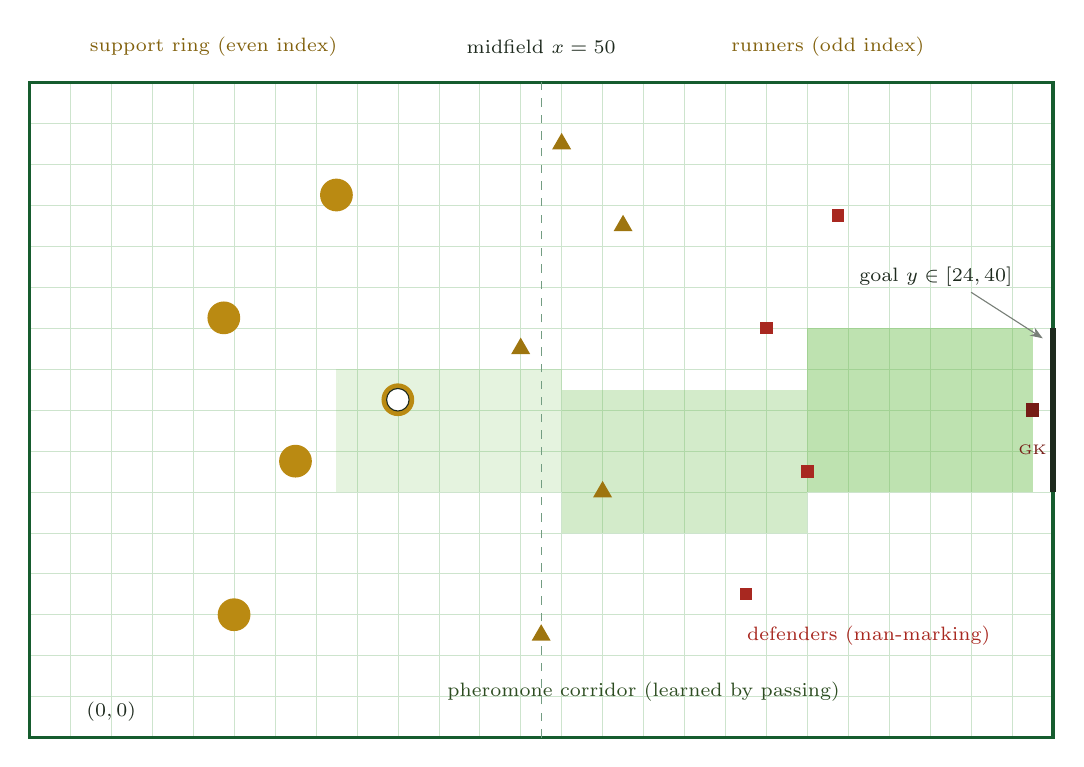
\begin{tikzpicture}[x=0.13cm,y=0.13cm]
  % pheromone grid
  \foreach \i in {0,4,...,100} \draw[green!30!gray!30, very thin] (\i,0) -- (\i,64);
  \foreach \j in {0,4,...,64} \draw[green!30!gray!30, very thin] (0,\j) -- (100,\j);
  % learned corridor (pheromone heat)
  \fill[pher, opacity=0.18] (30,24) rectangle (52,36);
  \fill[pher, opacity=0.30] (52,20) rectangle (76,34);
  \fill[pher, opacity=0.45] (76,24) rectangle (98,40);
  % pitch frame + goal
  \draw[very thick, pitch] (0,0) rectangle (100,64);
  \draw[line width=2.2pt, ink] (100,24) -- (100,40);
  \node[ink, font=\scriptsize, anchor=east] at (97,45) {goal $y\in[24,40]$};
  \draw[-{Stealth[length=1.6mm]}, thin, ink!60] (92,43.5) -- (99,39);
  \draw[dashed, pitch!60] (50,0) -- (50,64);
  % support (even idx) = gold circles
  \foreach \p in {(20,12),(26,27),(19,41),(30,53),(36,33)}
    \fill[gold] \p circle (1.6);
  % runners (odd idx) = gold triangles
  \foreach \p in {(50,10),(56,24),(48,38),(58,50),(52,58)}
    \node[regular polygon, regular polygon sides=3, fill=gold!85!black, inner sep=1.4pt] at \p {};
  % defenders = red squares
  \foreach \p in {(70,14),(76,26),(72,40),(79,51)}
    \node[rectangle, fill=defred, minimum size=4.5pt, inner sep=0pt] at \p {};
  % keeper
  \node[rectangle, fill=defred!70!black, minimum size=5pt, inner sep=0pt] at (98,32) {};
  \node[below=0pt, font=\tiny, defred!70!black] at (98,29.5) {GK};
  % ball
  \fill[white, draw=ink] (36,33) circle (1.1);
  % labels
  \node[gold!70!black, font=\scriptsize] at (18,67.5) {support ring (even index)};
  \node[gold!70!black, font=\scriptsize] at (78,67.5) {runners (odd index)};
  \node[defred, font=\scriptsize] at (82,10) {defenders (man-marking)};
  \node[pher!40!black, font=\scriptsize, align=center] at (60,4.5) {pheromone corridor (learned by passing)};
  \node[ink, font=\scriptsize] at (8,2.5) {$(0,0)$};
  \node[ink, font=\scriptsize] at (50,67.5) {midfield $x=50$};
\end{tikzpicture}
\caption{The micro-world: a $100\times64$ pitch discretized by a $25\times16$ pheromone grid
(cells of $4\times4$ units). Gold circles are support players, gold triangles are deep runners
(the caste split of \S\ref{sec:pso}), red squares are defenders, and the keeper guards the goal
mouth. The green wash sketches a pheromone corridor of the kind visible in the dashboard heatmap:
completed passes deposit trail, goals reinforce it, evaporation fades it.}
\label{fig:pitch}
\end{figure}

\subsection{The asymmetry: every attacker worse than every defender}

The experiment is only meaningful if the individuals are genuinely inferior, so the handicaps are
explicit and severe (Table~\ref{tab:asym}).

\begin{table}[H]
\centering
\caption{Designed asymmetry between attackers and defenders.}
\label{tab:asym}
\small
\begin{tabular}{@{}llll@{}}
\toprule
\textbf{Attribute} & \textbf{Shaolin attacker} & \textbf{Defender} & \textbf{Ratio}\\
\midrule
Top speed & $0.5$ u/tick ($0.38$ dribbling) & $0.68$ u/tick & $0.74\times$\\
Kick accuracy & $\sigma \propto$ distance, Eq.~\eqref{eq:sigma} & --- & ---\\
Vision & myopic, radius $15$ & full field & ---\\
Organization & none built-in & marking + presser + keeper & ---\\
Numbers & $10$ & $4$ + keeper & $2\times$\\
\bottomrule
\end{tabular}

\smallskip
{\footnotesize Numerical superiority is the attackers' only asset --- and exploiting it requires coordination.}
\end{table}

The single most important physical law of the world is that \textbf{aim error grows linearly
with kick distance}. A kick toward a point at distance $d$ has its direction perturbed by a
Gaussian angular error
\begin{equation}\label{eq:sigma}
  \theta \sim \mathcal{N}\!\bigl(0,\ \sigma(d)^2\bigr), \qquad
  \sigma(d) = 0.011 \cdot d \cdot \eta,
\end{equation}
where $\eta$ is the \emph{kick-noise} dial (default $1$). Since the lateral miss at the target
scales like $d\sigma(d) \propto d^2$, a $60$-unit shot is roughly $25\times$ less precise at its
target than a $12$-unit pass. This one fact creates the ecological niche for cooperation: a relay
of short, accurate passes can do what no long heroic ball can (Figure~\ref{fig:sigma}).

\begin{figure}[H]
\centering
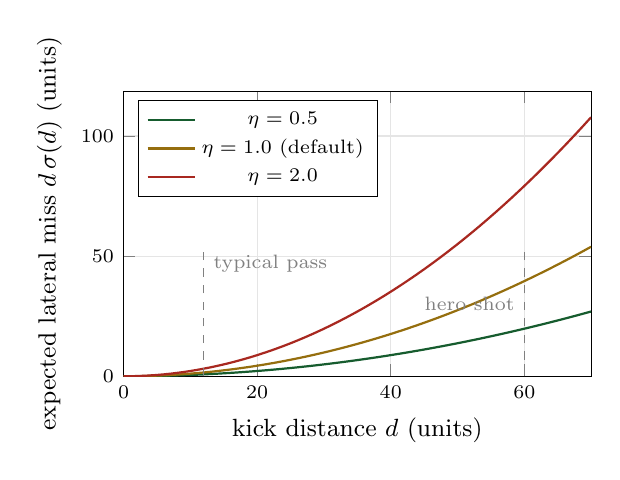
\begin{tikzpicture}
\begin{axis}[
  width=0.62\textwidth, height=5.2cm,
  xlabel={kick distance $d$ (units)}, ylabel={expected lateral miss $d\,\sigma(d)$ (units)},
  xmin=0, xmax=70, ymin=0,
  legend pos=north west, legend style={font=\scriptsize},
  grid=major, grid style={gray!20},
  tick label style={font=\scriptsize}, label style={font=\small},
]
\addplot[pitch, thick, domain=0:70, samples=60] {0.011*x*x*0.5}; \addlegendentry{$\eta=0.5$}
\addplot[gold!80!black, thick, domain=0:70, samples=60] {0.011*x*x*1.0}; \addlegendentry{$\eta=1.0$ (default)}
\addplot[defred, thick, domain=0:70, samples=60] {0.011*x*x*2.0}; \addlegendentry{$\eta=2.0$}
\draw[dashed, gray] (axis cs:12,0) -- (axis cs:12,55) node[pos=0.85, right, font=\scriptsize, gray] {typical pass};
\draw[dashed, gray] (axis cs:60,0) -- (axis cs:60,55) node[pos=0.55, left, font=\scriptsize, gray] {hero shot};
\end{axis}
\end{tikzpicture}
\caption{The physics that rewards cooperation: expected lateral miss grows \emph{quadratically}
with kick distance ($\sigma$ linear in $d$, miss $\approx d\sigma$). Five 12-unit passes stay
accurate where one 60-unit punt sprays wide.}
\label{fig:sigma}
\end{figure}

\subsection{Parameters}

\begin{table}[H]
\centering
\caption{Complete simulation parameters (defaults; all exposed as UI sliders or constructor options).}
\label{tab:params}
\small
\begin{tabular}{@{}llp{7.2cm}@{}}
\toprule
\textbf{Symbol / name} & \textbf{Default} & \textbf{Meaning}\\
\midrule
$W\times H$ & $100\times64$ & pitch dimensions\\
$n$ (\texttt{nPlayers}) & $10$ & attackers\\
\texttt{nDefenders} & $4$ (+keeper) & defenders\\
$v_a$ / $v_{drib}$ & $0.5$ / $0.38$ & attacker run / dribble speed (u/tick)\\
$v_d$ & $0.68\cdot k$ & defender speed; $k$ = \texttt{defSkill}\\
$v_{pass}$ / $v_{shot}$ & $1.7$ / $2.6$ & ball speed for passes / shots\\
$R_{kick}$ & $30$ & maximum pass range\\
$g$ (\texttt{shootGate}) & $1.15$ & shoot radius $= g\cdot R_{kick}$\\
$\eta$ (\texttt{kickNoise}) & $1.0$ & aim-noise multiplier in Eq.~\eqref{eq:sigma}\\
$r_{vis}$ (\texttt{vision}) & $15$ & attacker vision radius\\
$\rho$ (\texttt{evap}) & $0.0015$ & pheromone evaporation per tick\\
grid & $25\times16$ & pheromone cells ($4\times4$ units each)\\
$\tau_{max}$ & $3$ & pheromone cap per cell\\
\texttt{interceptP} & $0.22$ & per-tick interception probability in reach\\
\texttt{keeperReach} & $2.5\cdot k$ & save radius along the goal mouth\\
$T_{max}$ & $1200$ & episode timeout (ticks)\\
$R_{react}$ & $\max(3,\mathrm{round}(14/k))$ & defender re-marking period (ticks)\\
seed & $42$ (tests: $3,4,5$) & mulberry32 RNG seed\\
\bottomrule
\end{tabular}
\end{table}

\subsection{Metrics and hypothesis}

Per condition we record: \textbf{goals}, \textbf{shots}, \textbf{shots on target},
\textbf{pass completion rate} $= \frac{\text{completed}}{\text{attempted}}$, saves, and
possession ticks. Bookkeeping is honest by construction: a kicker can never receive his own pass
in flight, and recovering one's own loose ball counts as a dribble, not a completed pass ---
without these rules the pass statistics would flatter the swarm.

\begin{hypothesis}\label{hyp:main}
With identical bodies and identical physics, the swarm controller scores at least $5\times$ more
goals than the selfish controller over $300$ episodes ($3$ seeds $\times$ $100$), and at least
$15$ in absolute terms.
\end{hypothesis}

Hypothesis~\ref{hyp:main} is not merely stated --- it is literally \texttt{assert}~\#4 of the
test suite (\S\ref{sec:impl}).

% ============================================================
\section{System Architecture}\label{sec:arch}
% ============================================================

The system is deliberately minimal: one headless simulation module, one single-file dashboard,
one Node test script, zero dependencies. Figure~\ref{fig:arch} shows the module architecture;
Figure~\ref{fig:tick} shows the per-tick pipeline.

\begin{figure}[H]
\centering
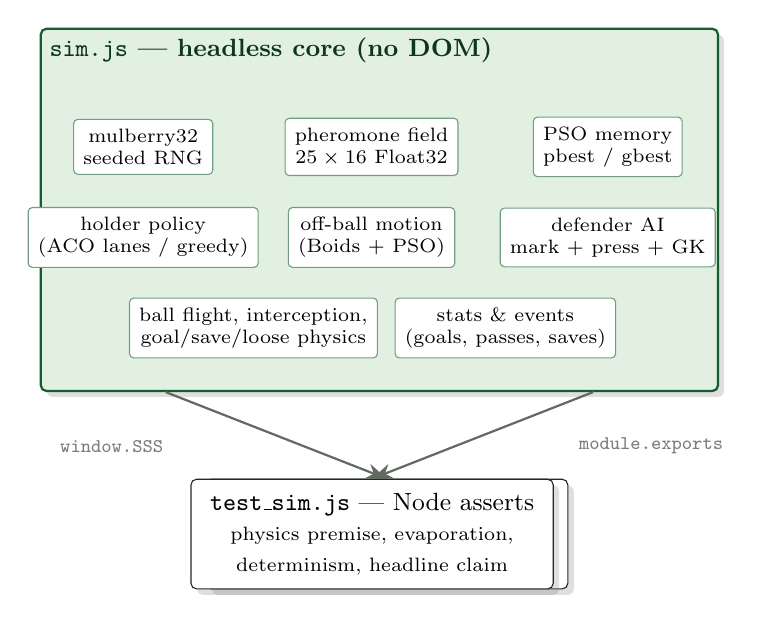
\begin{tikzpicture}[
  font=\small,
  box/.style={draw=ink, rounded corners=2pt, fill=white, align=center, inner sep=5pt, drop shadow={opacity=0.25}},
  core/.style={box, fill=pitchlight, draw=pitch, thick},
  sub/.style={draw=pitch!60, rounded corners=1.5pt, fill=white, align=center, inner sep=3.5pt, font=\scriptsize},
  arr/.style={-{Stealth[length=2.6mm]}, thick, ink!70},
]
% core
\node[core, minimum width=8.6cm, minimum height=4.6cm] (sim) at (0,0) {};
\node[anchor=north west, font=\bfseries\small, pitch!60!black] at (sim.north west) {\texttt{sim.js} --- headless core (no DOM)};
\node[sub] (rng) at (-3.0,0.8) {mulberry32\\seeded RNG};
\node[sub] (pher) at (-0.1,0.8) {pheromone field\\$25\times16$ Float32};
\node[sub] (pso) at (2.9,0.8) {PSO memory\\pbest / gbest};
\node[sub] (holder) at (-3.0,-0.35) {holder policy\\(ACO lanes / greedy)};
\node[sub] (boids) at (-0.1,-0.35) {off-ball motion\\(Boids + PSO)};
\node[sub] (def) at (2.9,-0.35) {defender AI\\mark + press + GK};
\node[sub] (ball) at (-1.6,-1.5) {ball flight, interception,\\goal/save/loose physics};
\node[sub] (stats) at (1.6,-1.5) {stats \& events\\(goals, passes, saves)};
% consumers
\node[box, below left=1.1cm and -2.4cm of sim.south, minimum width=4.6cm] (ui)
  {\texttt{index.html} --- dashboard\\ \scriptsize canvas pitch, heatmap overlay,\\ \scriptsize sliders, speed 0.25--4$\times$, benchmark};
\node[box, below right=1.1cm and -2.4cm of sim.south, minimum width=4.6cm] (test)
  {\texttt{test\_sim.js} --- Node asserts\\ \scriptsize physics premise, evaporation,\\ \scriptsize determinism, headline claim};
\draw[arr] (sim.south west)++(1.6,0) -- (ui.north);
\draw[arr] (sim.south east)++(-1.6,0) -- (test.north);
\node[font=\scriptsize, ink!60] at (-3.4,-3.0) {\texttt{window.SSS}};
\node[font=\scriptsize, ink!60] at (3.45,-3.0) {\texttt{module.exports}};
\end{tikzpicture}
\caption{Module architecture. The simulation core is UI-agnostic and exports the same API to the
browser (\texttt{window.SSS}) and to Node (\texttt{module.exports}); the dashboard and the test
suite are two thin consumers of one source of truth, so every visual claim is also a testable
claim.}
\label{fig:arch}
\end{figure}

\begin{figure}[H]
\centering
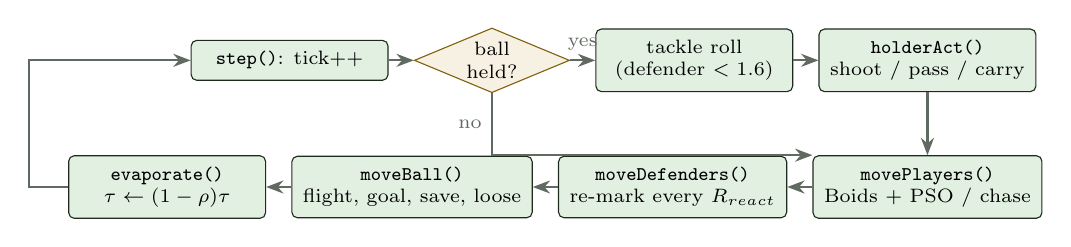
\begin{tikzpicture}[
  font=\scriptsize, node distance=3.2mm,
  st/.style={draw=ink, rounded corners=2pt, fill=pitchlight, align=center, inner sep=4pt, minimum width=2.5cm},
  dec/.style={draw=gold!70!black, fill=gold!12, diamond, aspect=2.4, align=center, inner sep=1pt},
  arr/.style={-{Stealth[length=2.2mm]}, thick, ink!70},
]
\node[st] (tick) {\texttt{step()}: tick++};
\node[dec, right=of tick] (held) {ball\\held?};
\node[st, right=of held] (tackle) {tackle roll\\(defender $<1.6$)};
\node[st, right=of tackle] (act) {\texttt{holderAct()}\\shoot / pass / carry};
\node[st, below=8mm of act] (move) {\texttt{movePlayers()}\\Boids + PSO / chase};
\node[st, left=of move] (defm) {\texttt{moveDefenders()}\\re-mark every $R_{react}$};
\node[st, left=of defm] (ballm) {\texttt{moveBall()}\\flight, goal, save, loose};
\node[st, left=of ballm] (evap) {\texttt{evaporate()}\\$\tau \leftarrow (1-\rho)\tau$};
\draw[arr] (tick) -- (held);
\draw[arr] (held) -- node[above]{yes} (tackle);
\draw[arr] (tackle) -- (act);
\draw[arr] (act) -- (move);
\draw[arr] (held) |- node[left, pos=0.25]{no} (move.north west);
\draw[arr] (move) -- (defm);
\draw[arr] (defm) -- (ballm);
\draw[arr] (ballm) -- (evap);
\draw[arr] (evap.west) -- ++(-0.5,0) |- ([yshift=0mm]tick.west);
\end{tikzpicture}
\caption{The per-tick pipeline. Every subsystem runs every tick; episode-ending events (goal,
tackle, interception, out-of-bounds, timeout) reset positions but --- crucially --- \emph{not}
the pheromone field or the PSO memories, which persist and accumulate across episodes.}
\label{fig:tick}
\end{figure}

\begin{remark}
The learning state (pheromone grid, pbest/gbest) surviving episode resets is what makes this a
\emph{learning} system rather than a reactive one: the team gets measurably better over the
first $\sim$60 episodes, visible in the learning curve of Figure~\ref{fig:learning}.
\end{remark}

% ============================================================
\section{Method: Three Algorithms, One Controller}\label{sec:method}
% ============================================================

The swarm controller decomposes the team's problem into three orthogonal sub-decisions, each
solved by one classic mechanism (Figure~\ref{fig:threeway}):

\begin{figure}[H]
\centering
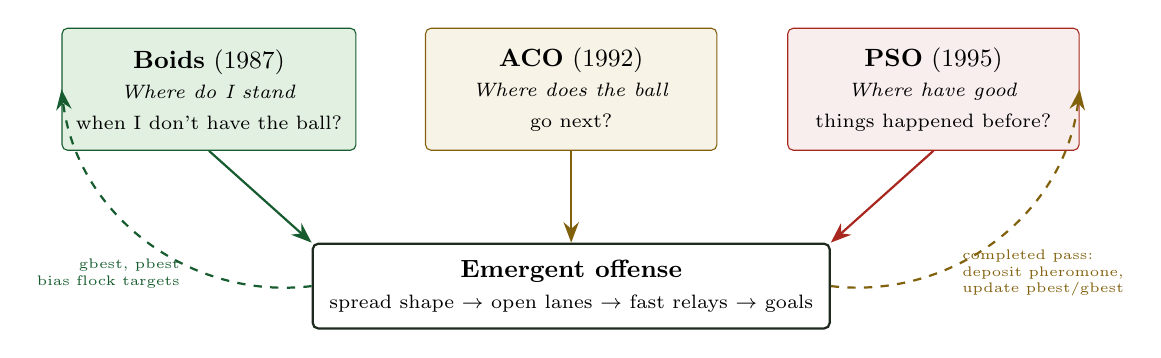
\begin{tikzpicture}[
  font=\small,
  mech/.style={draw, rounded corners=2pt, align=center, inner sep=5pt, minimum width=3.7cm, minimum height=1.55cm},
  arr/.style={-{Stealth[length=2.6mm]}, thick},
]
\node[mech, draw=pitch, fill=pitchlight] (boids) at (-4.6,0) {\textbf{Boids} (1987)\\ \scriptsize \emph{Where do I stand}\\ \scriptsize when I don't have the ball?};
\node[mech, draw=gold!70!black, fill=gold!10] (aco) at (0,0) {\textbf{ACO} (1992)\\ \scriptsize \emph{Where does the ball}\\ \scriptsize go next?};
\node[mech, draw=defred, fill=defred!8] (pso) at (4.6,0) {\textbf{PSO} (1995)\\ \scriptsize \emph{Where have good}\\ \scriptsize things happened before?};
\node[draw=ink, thick, rounded corners=2pt, fill=white, align=center, inner sep=6pt, minimum width=6.2cm] (emerge) at (0,-2.5)
  {\textbf{Emergent offense}\\ \scriptsize spread shape $\to$ open lanes $\to$ fast relays $\to$ goals};
\draw[arr, pitch] (boids.south) -- (emerge.north west);
\draw[arr, gold!70!black] (aco.south) -- (emerge.north);
\draw[arr, defred] (pso.south) -- (emerge.north east);
% feedback arrows
\draw[arr, gold!70!black, dashed] (emerge.east) to[bend right=45] node[pos=0.3, right=2mm, font=\tiny, align=left]{completed pass:\\deposit pheromone,\\update pbest/gbest} (pso.east);
\draw[arr, pitch, dashed] (emerge.west) to[bend left=45] node[pos=0.3, left=2mm, font=\tiny, align=right]{gbest, pbest\\bias flock targets} (boids.west);
\end{tikzpicture}
\caption{Division of labour and the feedback loop. Boids shapes the team, ACO routes the ball
through that shape, PSO remembers which spots paid off and feeds them back into the shape. Each
success (pass, goal) simultaneously updates the stigmergy field and the particle memories.}
\label{fig:threeway}
\end{figure}

\subsection{Boids: off-ball shape}\label{sec:boids}

Reynolds' three rules --- separation, cohesion, alignment --- govern every attacker who is not
holding or chasing the ball. For player $i$ at position $p_i$ the steering force is
\begin{equation}\label{eq:boids}
  F_i \;=\; 1.4\,F^{sep}_i \;+\; 1.1\,F^{coh}_i \;+\; F^{align}_i \;+\; w^{pso}_i\,F^{pso}_i ,
\end{equation}
with the components:

\begin{itemize}[itemsep=2pt]
  \item \textbf{Separation} pushes away from teammates within $9$ units \emph{and from
        defenders} within $6$ units. The defender term is caste-weighted (``bravery''): support
        players flee markers with weight $1.6$; runners hold their ground with weight $0.5$,
        because a runner who retreats from his marker has already lost the duel.
  \item \textbf{Cohesion toward a point that does not exist yet.} The flock anchor is not the
        ball but a point \emph{16 units ahead of it}, $a = (\min(W-6,\ x_{ball}+16),\ \cdot)$.
        The support ring therefore forms downfield of the ball, so that when a pass arrives
        the structure to relay it onward already exists. Players too far from the anchor are
        pulled in, players too close ($<7$) are pushed out --- a ring, not a cluster.
  \item \textbf{Alignment} is a constant drift toward the attacking end ($+x$), $0.6$ for
        runners, $0.35$ for support.
\end{itemize}

The resulting force is normalized and blended into the velocity with momentum,
$v \leftarrow 0.75\,v + 0.25\,\hat{F} v_a$, which smooths jitter and caps speed at $v_a=0.5$.
Figure~\ref{fig:boidsforces} illustrates the force composition on a single support player.

\begin{figure}[H]
\centering
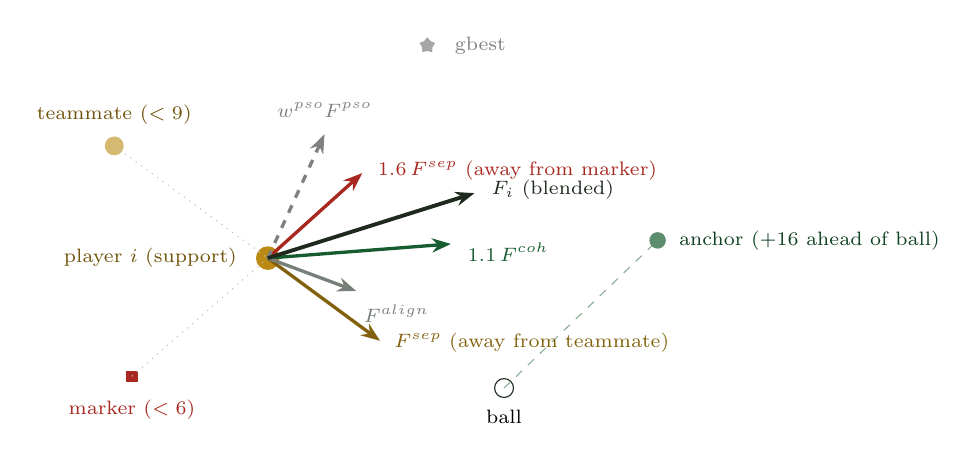
\begin{tikzpicture}[x=1.5cm,y=1.5cm, font=\scriptsize,
  arr/.style={-{Stealth[length=2.4mm]}, very thick}]
  % agent
  \fill[gold] (0,0) circle (0.10);
  \node[anchor=east, gold!60!black] at (-0.18,0) {player $i$ (support)};
  % sources (all west of the agent, so forces point east)
  \fill[gold!60] (-1.3,0.95) circle (0.08);
  \node[anchor=south, gold!60!black] at (-1.3,1.05) {teammate ($<9$)};
  \draw[gray!50, dotted] (-1.3,0.95) -- (0,0);
  \node[rectangle, fill=defred, minimum size=4pt, inner sep=0pt] at (-1.15,-1.0) {};
  \node[anchor=north, defred] at (-1.15,-1.12) {marker ($<6$)};
  \draw[gray!50, dotted] (-1.15,-1.0) -- (0,0);
  % ball + anchor (east)
  \fill[white, draw=ink] (2.0,-1.1) circle (0.08);
  \node[anchor=north] at (2.0,-1.2) {ball};
  \draw[pitch!50, dashed] (2.0,-1.1) -- (3.3,0.15);
  \fill[pitch!70] (3.3,0.15) circle (0.07);
  \node[anchor=west, pitch!70!black] at (3.4,0.15) {anchor ($+16$ ahead of ball)};
  % gbest (north-east)
  \node[star, star points=5, fill=gray!70, inner sep=1.4pt] at (1.35,1.8) {};
  \node[anchor=west, gray] at (1.5,1.8) {gbest};
  % forces, fanned so no two labels collide
  \draw[arr, gold!70!black] (0,0) -- (0.95,-0.70)
    node[anchor=west] at (0.98,-0.72) {$F^{sep}$ (away from teammate)};
  \draw[arr, defred] (0,0) -- (0.80,0.72)
    node[anchor=west] at (0.84,0.74) {$1.6\,F^{sep}$ (away from marker)};
  \draw[arr, pitch] (0,0) -- (1.55,0.12)
    node[anchor=west] at (1.60,0.05) {$1.1\,F^{coh}$};
  \draw[arr, ink!60] (0,0) -- (0.75,-0.28)
    node[anchor=north west] at (0.72,-0.30) {$F^{align}$};
  \draw[arr, gray, dashed] (0,0) -- (0.48,1.05)
    node[anchor=south] at (0.48,1.10) {$w^{pso} F^{pso}$};
  \draw[arr, ink, line width=1.4pt] (0,0) -- (1.75,0.55)
    node[anchor=west] at (1.80,0.58) {$F_i$ (blended)};
\end{tikzpicture}
\caption{Force composition on one off-ball support player, Eq.~\eqref{eq:boids}: separation from
a nearby teammate and (more strongly, weight 1.6) from a marking defender, cohesion toward the
ring anchor held \emph{ahead of} the ball, constant goalward alignment, and the normalized PSO
hint. The bold vector is the blended steering force.}
\label{fig:boidsforces}
\end{figure}

\subsection{ACO stigmergy: routing the ball}\label{sec:aco}

The pitch carries a $25\times16$ pheromone field $\tau$ (one \texttt{Float32} per $4\times4$
cell). The three ACO operators from the lecture map one-to-one onto game events:

\paragraph{Deposit.} When a pass from $A$ to $B$ is \emph{completed}, pheromone is laid along
the corridor by sampling the segment every 2 units:
\begin{equation}\label{eq:deposit}
  \tau_c \leftarrow \min\!\bigl(\tau_{max},\ \tau_c + \Delta\bigr), \qquad
  \Delta_{pass} = 0.12 + 0.25\,\frac{x_B}{W}, \qquad
  \Delta_{goal} = 0.9 .
\end{equation}
Deposits are \emph{quality-weighted}, exactly as the lecture prescribes (``good solutions receive
stronger pheromone''): passes deeper into enemy territory deposit more, and a goal reinforces its
origin corridor with $7\times$ the strength of an ordinary pass.

\paragraph{Evaporation.} Every tick, every cell decays: $\tau \leftarrow (1-\rho)\,\tau$ with
$\rho = 0.0015$. This is the lecture's exploration-preserving operator: corridors the defense has
learned to cover fade away instead of trapping the team forever (``prevents dependency on early
solutions'').

\paragraph{Probabilistic construction (roulette wheel).} When the holder $h$ considers pass
candidates $j$ within range $[3, R_{kick}]$, each lane is scored by pheromone $\times$
heuristic desirability:
\begin{equation}\label{eq:lane}
  S_{hj} = \bigl(0.4 + \bar\tau_{hj}\bigr)\,
           \bigl(0.45 + 0.55\,O_{hj}\bigr)\,
           \Bigl(1 + 1.6\,P_{hj} + 0.4\,C_{hj} + 0.6\,\tfrac{x_j}{W}\Bigr),
\end{equation}
where $\bar\tau_{hj}\in[0,1]$ is the capped mean pheromone along the lane, $O_{hj}\in[0,1]$ is
\emph{openness} (nearest defender's distance to the lane segment, saturating at $7$ units),
$P_{hj} = (x_j - x_h)/R_{kick}$ is field progress, and $C_{hj} = 1 - d_{hj}/R_{kick}$ rewards
short (accurate) balls. The target is then drawn by \textbf{roulette-wheel selection} with
weights $w_j = S_{hj}^{\,\beta}$, $\beta = 2$ --- the very selection operator from the GA part
of the lecture, with $\beta$ playing the role of selection pressure. Argmax was tried and
rejected; see \S\ref{sec:discussion}.

Two hard rules bound the stochastic policy: inside shot range ($d_{goal} < 1.15\,R_{kick}$) the
holder \emph{shoots} whenever the shooting lane is open, he is pressed, very close, or has held
too long --- otherwise pheromone loops would circulate the ball forever; and outside shot range
a brief one-touch window (up to 2 ticks, unpressed) lets play flow without giving the keeper
time to set. The full policy is Algorithm~\ref{alg:holder} and Figure~\ref{fig:holderflow}.

\begin{algorithm}[H]
\caption{Swarm holder policy (one tick, ball held by $h$)}\label{alg:holder}
\begin{algorithmic}[1]
\State $pressed \gets \exists\, d \in \mathcal{D}: \operatorname{dist}(d,h) < 5$;\quad $inRange \gets d_{goal} < 1.15\,R_{kick}$
\If{$holdTicks < 3$ \textbf{and not} $pressed$ \textbf{and not} $inRange$} \Return \Comment{one-touch flow}
\EndIf
\If{$inRange$} \Comment{shooting is a hard rule near goal}
  \State $t_y \gets$ far post from keeper;\quad $O \gets$ openness$(h \to (W, t_y))$
  \If{$O > 0.25$ \textbf{or} $d_{goal} < 12$ \textbf{or} $holdTicks > 12$ \textbf{or} $pressed$}
    \State \textbf{shoot} at $(W, t_y)$ with speed $2.6$; \Return
  \EndIf
\EndIf
\State build candidates $j$ with $3 < d_{hj} \le R_{kick}$; score $S_{hj}$ by Eq.~\eqref{eq:lane}
\If{candidates exist \textbf{and} ($pressed$ \textbf{or} $holdTicks > 16$ \textbf{or} $\max_j S_{hj} > 0.45$)}
  \State draw $j^\ast \sim$ roulette$(w_j = S_{hj}^2)$ \Comment{GA selection operator, $\beta=2$}
  \State add lead of up to $3$ units if $j^\ast$ is a forward runner \Comment{ball into space}
  \State \textbf{pass} to $j^\ast$ with speed $1.7$; \Return
\EndIf
\State \textbf{carry} toward goal at $0.38$ ($0.19$ if pressed) \Comment{nothing good yet}
\end{algorithmic}
\end{algorithm}

\begin{figure}[H]
\centering
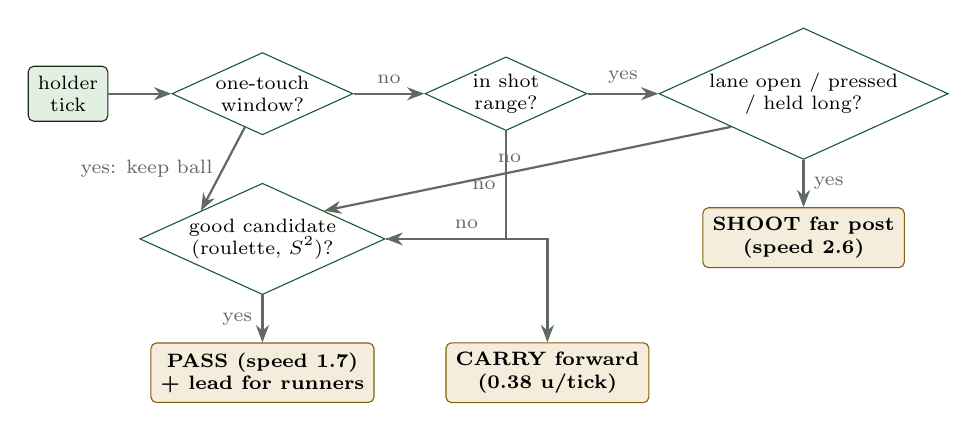
\begin{tikzpicture}[
  font=\scriptsize, node distance=2.6mm and 4.5mm,
  st/.style={draw=ink, rounded corners=2pt, fill=pitchlight, align=center, inner sep=3.5pt},
  act/.style={draw=gold!70!black, rounded corners=2pt, fill=gold!15, align=center, inner sep=3.5pt, font=\scriptsize\bfseries},
  dec/.style={draw=pitch, fill=white, diamond, aspect=2.2, align=center, inner sep=0.5pt},
  arr/.style={-{Stealth[length=2.2mm]}, thick, ink!70},
]
\node[dec] (one) {one-touch\\window?};
\node[dec, right=9mm of one] (rng) {in shot\\range?};
\node[dec, right=9mm of rng] (open) {lane open / pressed\\/ held long?};
\node[act, below=6mm of open] (shoot) {SHOOT far post\\(speed 2.6)};
\node[dec, below=6mm of one] (cand) {good candidate\\(roulette, $S^2$)?};
\node[act, below=6mm of cand] (pass) {PASS (speed 1.7)\\+ lead for runners};
\node[act, right=9mm of pass] (carry) {CARRY forward\\(0.38 u/tick)};
\node[st, left=8mm of one] (in) {holder\\tick};
\draw[arr] (in) -- (one);
\draw[arr] (one) -- node[above]{no} (rng);
\draw[arr] (one) -- node[left]{yes: keep ball} (cand.north west);
\draw[arr] (rng) -- node[above]{yes} (open);
\draw[arr] (open) -- node[right]{yes} (shoot);
\draw[arr] (rng) |- node[left, pos=0.25]{no} (cand);
\draw[arr] (open.south west) -- node[above left=-2pt]{no} (cand.north east);
\draw[arr] (cand) -- node[left]{yes} (pass);
\draw[arr] (cand) -| node[above, pos=0.25]{no} (carry);
\end{tikzpicture}
\caption{Holder decision flow (swarm mode). The stochastic ACO core (roulette over
pheromone-weighted lanes) is sandwiched between two deterministic guards: a one-touch window
that keeps play fast, and a hard shooting rule that prevents infinite pheromone circulation.}
\label{fig:holderflow}
\end{figure}

\subsection{PSO: spatial memory and the caste split}\label{sec:pso}

Each player's off-ball \emph{positioning target} is treated as a particle. Whenever player $i$
receives a pass at $p$, the reception is valued by proximity to goal,
$val = 1 - \operatorname{dist}(p, \text{goal})/110$, and the memories update exactly as in the
lecture's ``dual experience learning'':
\[
  val > pbestVal_i \;\Rightarrow\; pbest_i \leftarrow p, \qquad
  val > gbest.val \;\Rightarrow\; gbest \leftarrow p .
\]
A goal overrides $gbest$ with the shot's origin at full value $1$ --- the single most
informative event in the game. The PSO steering hint for player $i$ is the classic two-attractor
velocity rule,
\begin{equation}\label{eq:pso}
  F^{pso}_i = c_1 r_1 (pbest_i - p_i) + c_2 r_2 (gbest - p_i), \qquad r_1, r_2 \sim U(0,1),
\end{equation}
\emph{normalized to at most unit length} before entering Eq.~\eqref{eq:boids} --- PSO is a
directional hint, not a command (see the negative result in \S\ref{sec:discussion}).

\paragraph{Caste split as diversity preservation.} The lecture warns that a population which
becomes too uniform converges prematurely. Here the failure mode is spatial: if all ten players
chase the same $gbest$, the team collapses onto one point and the passing web dies. The remedy
is a fixed caste split, in the spirit of ant workers/soldiers:
\begin{center}
\small
\begin{tabular}{@{}lcc@{}}
\toprule
 & \textbf{Runners (odd index)} & \textbf{Support (even index)}\\
\midrule
PSO weights $(c_1, c_2)$ & $(0.8,\ 0.3)$ --- trust own pbest & $(0.3,\ 0.7)$ --- follow gbest\\
PSO blend $w^{pso}$ & $0.9$ & $0.4$\\
Marker bravery & $0.5$ (hold ground) & $1.6$ (escape)\\
Goalward drift & $0.6$ & $0.35$\\
Spawn & already upfield ($x \in [45,62]$) & deep ($x \in [15,45]$)\\
Role & stretch the defense deep & keep the relay ring\\
\bottomrule
\end{tabular}
\end{center}
Runners weighting $pbest$ is \emph{diversity} (ten different beliefs about where the good spots
are); support weighting $gbest$ is \emph{consensus} (a coherent ring around the proven corridor).
Initialization is optimistic and diverse: each player starts believing in his own random spot in
the final third ($pbestVal \approx 0.65$--$0.77$, the value of a final-third reception), so
ordinary midfield receptions cannot overwrite the ambition --- a direct antidote to the
``midfield anchor'' collapse described in \S\ref{sec:discussion}.

\subsection{The selfish baseline}

The baseline is the same code path with all three mechanisms removed. The holder dribbles
straight at goal and shoots the instant $d_{goal} < R_{kick}$; every other player chases the
ball if he can see it (vision radius $15$) and wanders randomly if not. This is not a parody ---
it is a faithful implementation of ``every agent individually optimizes the obvious objective,''
and its failure is instructive: it attempts long shots from $\sim$30 units where
Eq.~\eqref{eq:sigma} gives them no chance, and its pass completion is exactly $0\%$ because it
never intends a pass at all.

\subsection{The opposition}

The defense is deliberately competent. One defender (the nearest) \emph{presses} the ball; the
others man-mark the nearest unmarked attackers, standing goal-side ($+2.5$ in $x$). Marks are
re-assigned every $R_{react} = \max(3, \operatorname{round}(14/k))$ ticks --- a realistic
cognitive cycle that the swarm learns to exploit (\S\ref{sec:whywin}). The keeper tracks the
ball's $y$ along the goal mouth at up to $0.45k$/tick and saves shots within reach $2.5k$;
parried shots rebound into the box as loose balls. Interception of a moving ball is
probabilistic ($p = 0.22k$ per tick within $1.25k$ units), so well-hit through-balls can thread
a crowd --- and badly chosen ones die.

% ============================================================
\section{Implementation and Verification}\label{sec:impl}
% ============================================================

\subsection{Determinism as a scientific instrument}

All randomness flows through a single seeded mulberry32 generator; Gaussian noise is produced by
Box--Muller from the same stream. Consequently every run is bit-reproducible: the headline
result is not ``what we happened to observe'' but a permanent property of seeds $\{3,4,5\}$ that
anyone can re-derive with \texttt{node test\_sim.js}.

\begin{lstlisting}[language=JavaScript, caption={The two physical laws the whole thesis rests on: seeded determinism and distance-proportional aim error.}]
function mulberry32(seed) { /* deterministic 32-bit stream */ }
// Aim error: sigma (radians) grows linearly with kick distance.
// This single physical fact is why short-pass relays beat long solo shots.
function kickSigma(dist, noise) { return 0.011 * dist * noise; }
\end{lstlisting}

\subsection{The test suite: claims as assertions}

\texttt{test\_sim.js} contains exactly four checks --- the smallest set that fails if the thesis
breaks:

\begin{enumerate}[itemsep=2pt]
  \item \textbf{Physics premise:} $\sigma(25) > 2\,\sigma(8)$ --- error must grow with distance,
        else the niche for cooperation does not exist.
  \item \textbf{Evaporation:} a pheromone cell decays below $0.4$ after 100 ticks at
        $\rho = 0.01$ --- the exploration operator works.
  \item \textbf{Determinism:} two swarm runs with seed 7 produce identical goal counts.
  \item \textbf{The claim} (Hypothesis~\ref{hyp:main}): over $3\times100$ episodes,
        $\text{swarm} \ge 15$ goals and $\text{swarm} \ge 5\times\max(1,\text{selfish})$.
\end{enumerate}

\noindent Output on the submitted code:
\begin{lstlisting}[language={}, numbers=none]
$ node test_sim.js
selfish: 1/300 goals, swarm: 17/300 goals
swarm pass completion: 95.3%
all tests pass
\end{lstlisting}

\subsection{The dashboard}

\texttt{index.html} is a single-file, zero-dependency visualization: live canvas pitch with the
pheromone heatmap overlay (toggleable), swarm/selfish mode switch on identical players, a
playback-speed slider ($0.25\times$--$4\times$) with a ball motion trail, parameter sliders
(team size, kick noise, vision, evaporation, defender skill), live metrics, and a one-click
300-episode benchmark reproducing the test-suite numbers with a comparison chart
(Figure~\ref{fig:dashboard}).

\begin{figure}[H]
\centering
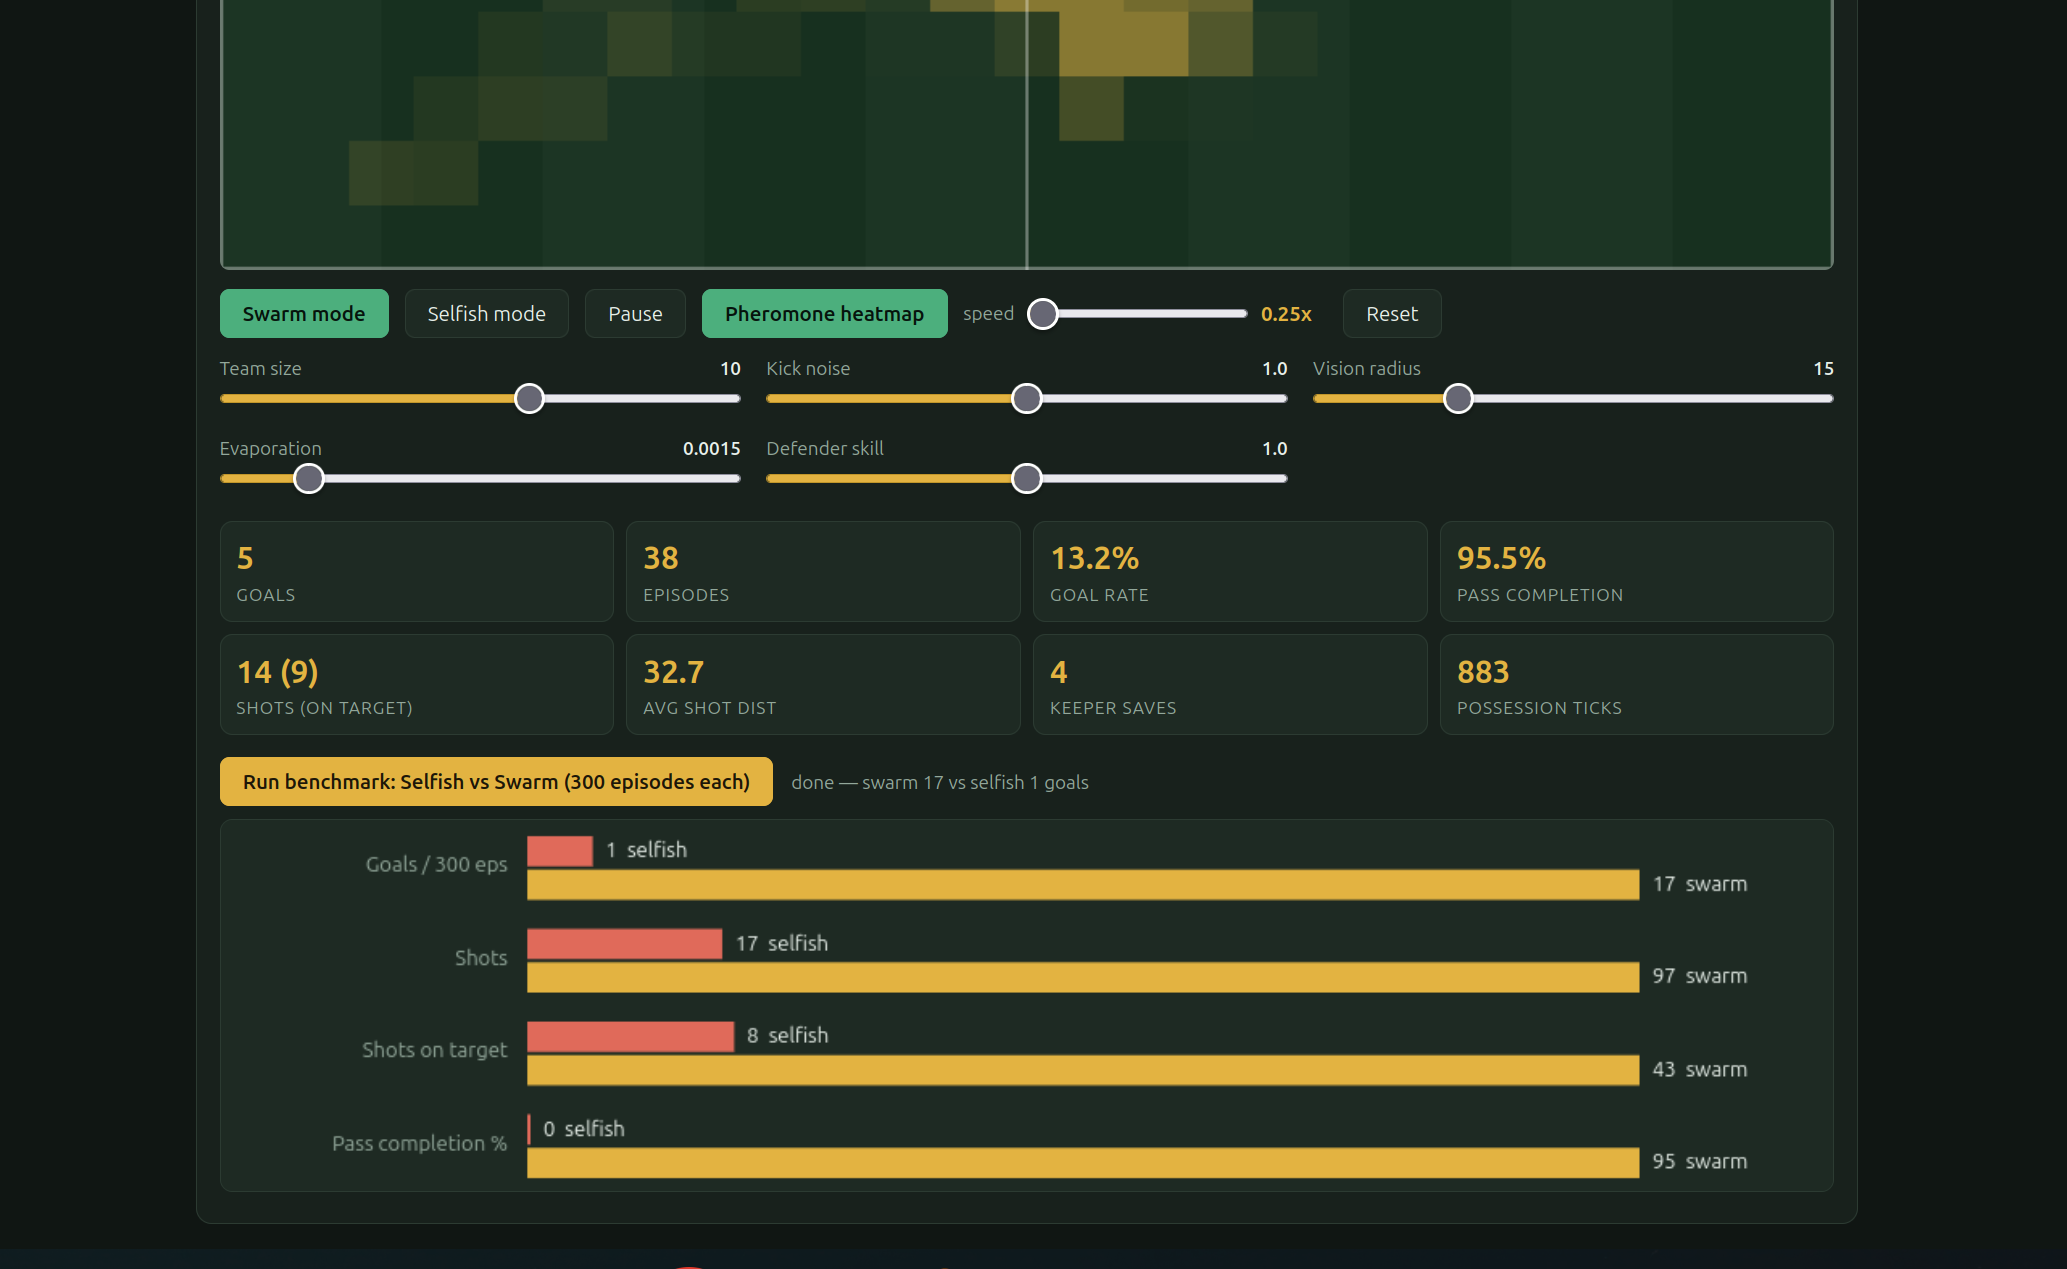
\includegraphics[width=0.9\textwidth]{screenshot.png}
\caption{The dashboard after a 300-episode benchmark: goals 17 vs 1, shots 97 vs 17, shots on
target 43 vs 8, pass completion 95\% vs 0\%. The glowing overlay on the pitch is the live
pheromone field --- the corridors the team has collectively learned.}
\label{fig:dashboard}
\end{figure}

% ============================================================
\section{Experiments and Results}\label{sec:results}
% ============================================================

\subsection{Protocol}

Unless stated otherwise, every number below aggregates \textbf{3 seeds $\times$ 100 episodes}
(seeds 3, 4, 5) per configuration, so that no single lucky seed can flip a verdict. Learning
state persists within a run and is reset between runs.

\subsection{Headline result}

\begin{table}[H]
\centering
\caption{Headline benchmark, 300 episodes per mode, identical seeds and physics.}
\label{tab:headline}
\begin{tabular}{@{}lcccc@{}}
\toprule
\textbf{Controller} & \textbf{Goals} & \textbf{Shots} & \textbf{On target} & \textbf{Pass completion}\\
\midrule
Swarm (Boids + ACO + PSO) & \textbf{17} & 97 & 43 & \textbf{95.3\%}\\
Selfish baseline          & 1           & 17 & 8  & 0.0\%\\
\midrule
Ratio & $17\times$ & $5.7\times$ & $5.4\times$ & ---\\
\bottomrule
\end{tabular}
\end{table}

\begin{figure}[H]
\centering
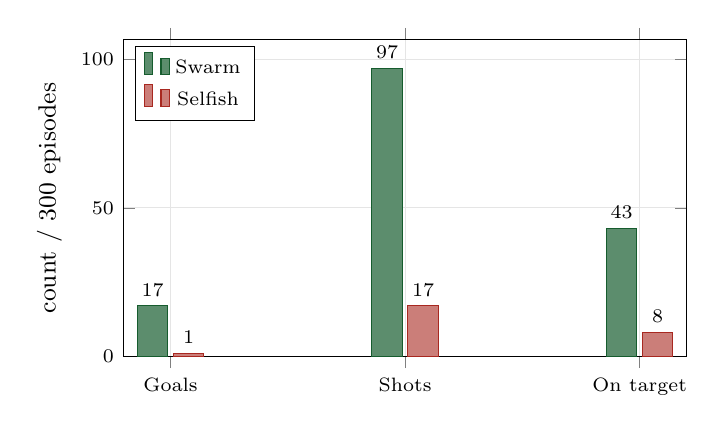
\begin{tikzpicture}
\begin{axis}[
  ybar, bar width=11pt,
  width=0.72\textwidth, height=5.6cm,
  symbolic x coords={Goals, Shots, On target},
  xtick=data, ymin=0,
  ylabel={count / 300 episodes},
  legend style={font=\scriptsize, at={(0.02,0.98)}, anchor=north west},
  nodes near coords, every node near coord/.append style={font=\scriptsize},
  tick label style={font=\scriptsize}, label style={font=\small},
  grid=major, grid style={gray!20},
]
\addplot[fill=pitch!70, draw=pitch] coordinates {(Goals,17) (Shots,97) (On target,43)};
\addplot[fill=defred!60, draw=defred] coordinates {(Goals,1) (Shots,17) (On target,8)};
\legend{Swarm, Selfish}
\end{axis}
\end{tikzpicture}
\caption{Headline benchmark. The swarm does not merely convert better --- it manufactures
$5.7\times$ more shots in the first place, because relays deliver the ball into range where solo
dribbles are tackled long before arrival.}
\label{fig:headlinebar}
\end{figure}

Hypothesis~\ref{hyp:main} is confirmed with margin: $17 \ge 15$ and $17 \ge 5\times1$. Across a
wider seed sweep the swarm averages roughly $9 \pm 3$ goals per 150 episodes while the selfish
baseline stays at 0--1; the advantage is structural, not seed luck.

\subsection{Learning curve: the colony converges}

Figure~\ref{fig:learning} plots cumulative goals against episode index, summed over the three
seeds. The swarm's curve is convex: about 6 goals in the first 55 episodes, then 11 more in the
remaining 45. This acceleration is the ACO convergence story from the lecture made visible ---
early episodes explore corridors nearly blind; as pheromone accumulates on lanes the defense
fails to cover and $gbest$ locks onto proven shooting origins, the same weak bodies score at
almost twice their early rate. The selfish baseline, having no memory of any kind, stays flat.

\begin{figure}[H]
\centering
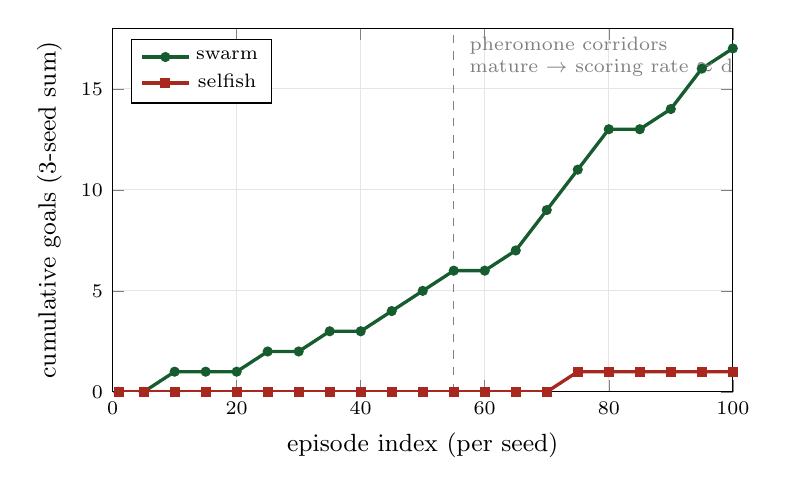
\begin{tikzpicture}
\begin{axis}[
  width=0.78\textwidth, height=6.2cm,
  xlabel={episode index (per seed)}, ylabel={cumulative goals (3-seed sum)},
  xmin=0, xmax=100, ymin=0, ymax=18,
  legend pos=north west, legend style={font=\scriptsize},
  grid=major, grid style={gray!20},
  tick label style={font=\scriptsize}, label style={font=\small},
]
\addplot[pitch, very thick, mark=*, mark size=1.2pt] coordinates {
(1,0) (5,0) (10,1) (15,1) (20,1) (25,2) (30,2) (35,3) (40,3) (45,4) (50,5) (55,6) (60,6) (65,7) (70,9) (75,11) (80,13) (85,13) (90,14) (95,16) (100,17)
};
\addlegendentry{swarm}
\addplot[defred, very thick, mark=square*, mark size=1.2pt] coordinates {
(1,0) (5,0) (10,0) (15,0) (20,0) (25,0) (30,0) (35,0) (40,0) (45,0) (50,0) (55,0) (60,0) (65,0) (70,0) (75,1) (80,1) (85,1) (90,1) (95,1) (100,1)
};
\addlegendentry{selfish}
\draw[dashed, gray] (axis cs:55,0) -- (axis cs:55,18);
\node[font=\scriptsize, gray, anchor=west, align=left] at (axis cs:56,16.6) {pheromone corridors\\mature $\to$ scoring rate $\approx$ doubles};
\end{axis}
\end{tikzpicture}
\caption{Cumulative goals vs.\ episode index (3-seed sum). The convex swarm curve is stigmergic
learning: pheromone and PSO memory persist across episodes, so the team improves with no change
to any individual. The memoryless selfish baseline is flat.}
\label{fig:learning}
\end{figure}

\subsection{Kick noise: the thesis in one dial}

Raising $\eta$ scales all aim error. Table \& Figure~\ref{fig:noise}: the selfish baseline is
already dead at every noise level (its 30-unit shots miss even at $\eta = 0.5$), while the swarm
degrades \emph{gracefully} --- pass completion falls only from 97.3\% to 88.6\% as noise sextuples,
because 12-unit passes have little error to amplify. Coordination is not just stronger; it is
\emph{more robust to physical degradation}, which is the deeper claim.

\begin{figure}[H]
\centering
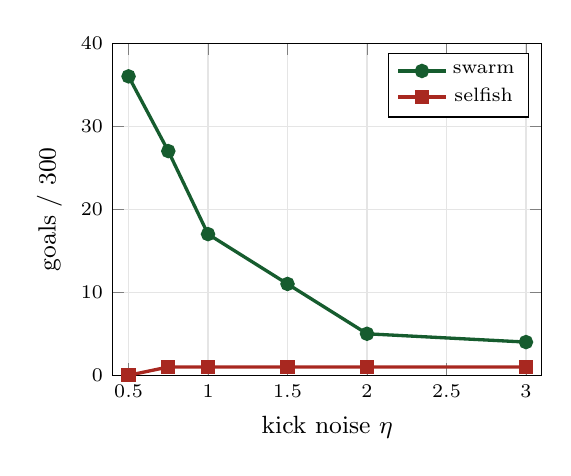
\begin{tikzpicture}
\begin{axis}[
  width=0.58\textwidth, height=5.8cm,
  xlabel={kick noise $\eta$}, ylabel={goals / 300},
  xmin=0.4, xmax=3.1, ymin=0, ymax=40,
  legend pos=north east, legend style={font=\scriptsize},
  grid=major, grid style={gray!20},
  tick label style={font=\scriptsize}, label style={font=\small},
]
\addplot[pitch, very thick, mark=*] coordinates {(0.5,36) (0.75,27) (1.0,17) (1.5,11) (2.0,5) (3.0,4)};
\addlegendentry{swarm}
\addplot[defred, very thick, mark=square*] coordinates {(0.5,0) (0.75,1) (1.0,1) (1.5,1) (2.0,1) (3.0,1)};
\addlegendentry{selfish}
\end{axis}
\end{tikzpicture}%
\hfill
\begin{minipage}[b]{0.4\textwidth}
\centering
\small
\begin{tabular}{@{}ccc@{}}
\toprule
$\eta$ & swarm pass\% & swarm goals\\
\midrule
0.5 & 97.3 & 36\\
0.75 & 96.3 & 27\\
1.0 & 95.3 & 17\\
1.5 & 92.8 & 11\\
2.0 & 92.4 & 5\\
3.0 & 88.6 & 4\\
\bottomrule
\end{tabular}
\vspace{6mm}
\end{minipage}
\caption{Kick-noise sweep. The selfish strategy has no regime in which it works; the swarm
degrades gracefully because short passes tolerate noise (Eq.~\eqref{eq:sigma} punishes
distance, and relays keep distances short).}
\label{fig:noise}
\end{figure}

\subsection{Evaporation: exploration vs.\ memory}

The lecture presents evaporation as the balance knob between remembering and re-exploring.
The sweep (Figure~\ref{fig:evapsweep}) confirms a broad optimum at small $\rho$: with
$\rho \lesssim 0.0015$ the field retains corridor knowledge across episodes (17--19 goals);
at $\rho = 0.02$ memory fades faster than the team can rebuild it and goals drop to 10. At the
extreme $\rho = 0.08$ the pheromone term is effectively dead --- yet the team still scores 16,
revealing that the heuristic part of Eq.~\eqref{eq:lane} (openness, progress, shortness) plus
Boids shape and PSO memory carry much of the load. Stigmergy is an amplifier here, not a
single point of failure --- an ablation insight we did not design for but the sweep exposed.

\begin{figure}[H]
\centering
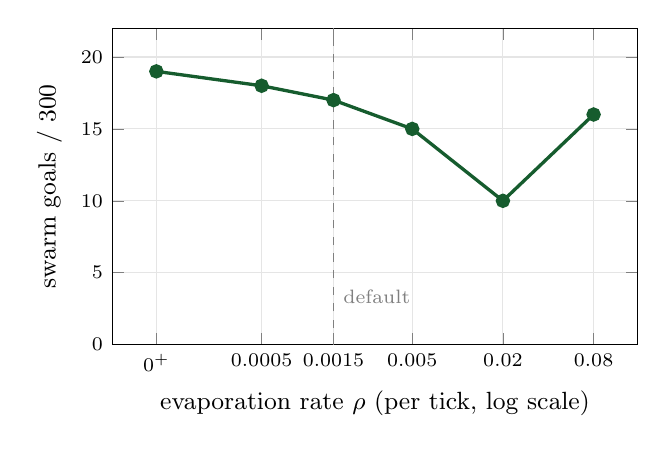
\begin{tikzpicture}
\begin{semilogxaxis}[
  width=0.68\textwidth, height=5.6cm,
  xlabel={evaporation rate $\rho$ (per tick, log scale)}, ylabel={swarm goals / 300},
  ymin=0, ymax=22,
  grid=major, grid style={gray!20},
  tick label style={font=\scriptsize}, label style={font=\small},
  xtick={0.0001,0.0005,0.0015,0.005,0.02,0.08},
  xticklabels={$0^{+}$,0.0005,0.0015,0.005,0.02,0.08},
]
\addplot[pitch, very thick, mark=*] coordinates {(0.0001,19) (0.0005,18) (0.0015,17) (0.005,15) (0.02,10) (0.08,16)};
\draw[dashed, gray] (axis cs:0.0015,0) -- (axis cs:0.0015,22) node[pos=0.15, right, font=\scriptsize, gray] {default};
\end{semilogxaxis}
\end{tikzpicture}
\caption{Evaporation sweep ($\rho=0$ plotted at $10^{-4}$). Small $\rho$ preserves cross-episode
corridor memory; $\rho=0.02$ erases it faster than play rebuilds it. The partial recovery at
$\rho=0.08$ shows the heuristic + Boids + PSO scaffolding scores even with stigmergy effectively
ablated.}
\label{fig:evapsweep}
\end{figure}

\subsection{Team size: cooperation needs critical mass}

Swarm intelligence should require a swarm. Figure~\ref{fig:teamsize}: at $n = 4$--$6$ the two
controllers are indistinguishable (1--4 goals each) --- too few bodies to form a ring \emph{and}
staff deep runs, so the ``web'' never exists. From $n = 8$ the collective advantage switches on
sharply ($15$ vs $2$) and keeps growing at $n = 12$ ($23$ vs $2$). Coordination is an emergent,
threshold phenomenon: below critical mass, structure cannot pay for itself.

\begin{figure}[H]
\centering
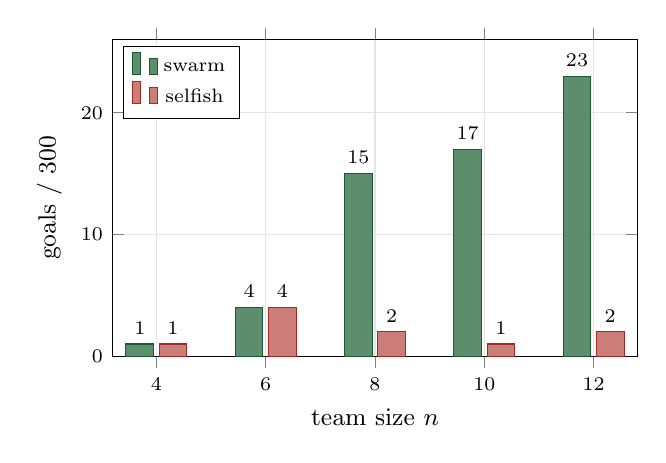
\begin{tikzpicture}
\begin{axis}[
  ybar, bar width=10pt,
  width=0.68\textwidth, height=5.6cm,
  xlabel={team size $n$}, ylabel={goals / 300},
  symbolic x coords={4,6,8,10,12}, xtick=data,
  ymin=0, ymax=26,
  legend style={font=\scriptsize, at={(0.02,0.98)}, anchor=north west},
  nodes near coords, every node near coord/.append style={font=\scriptsize},
  tick label style={font=\scriptsize}, label style={font=\small},
  grid=major, grid style={gray!20},
]
\addplot[fill=pitch!70, draw=pitch] coordinates {(4,1) (6,4) (8,15) (10,17) (12,23)};
\addplot[fill=defred!60, draw=defred] coordinates {(4,1) (6,4) (8,2) (10,1) (12,2)};
\legend{swarm, selfish}
\end{axis}
\end{tikzpicture}
\caption{Team-size sweep. Below $n\approx8$ the swarm cannot simultaneously maintain a support
ring and deep runners, and coordination confers nothing; above the threshold the advantage
appears abruptly and grows. Emergence has a critical mass.}
\label{fig:teamsize}
\end{figure}

\subsection{Defender skill: the advantage that survives}

Scaling defender speed, reactions, reach and interception together (Figure~\ref{fig:defskill}):
against weak defenders ($k = 0.7$) both controllers score, but the swarm still leads $58$ to
$14$. As $k$ rises the selfish baseline is extinguished entirely ($0$ from $k = 1.15$) while the
swarm keeps scoring even at $k = 1.3$ ($6$ goals). The swarm's edge is largest \emph{relative to
what is achievable} exactly where the problem is hardest --- coordination is how weak agents
survive strong opposition.

\begin{figure}[H]
\centering
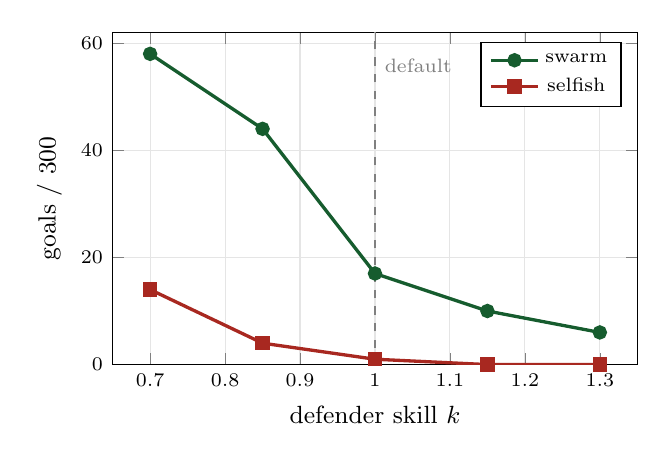
\begin{tikzpicture}
\begin{axis}[
  width=0.68\textwidth, height=5.8cm,
  xlabel={defender skill $k$}, ylabel={goals / 300},
  xmin=0.65, xmax=1.35, ymin=0, ymax=62,
  legend pos=north east, legend style={font=\scriptsize},
  grid=major, grid style={gray!20},
  tick label style={font=\scriptsize}, label style={font=\small},
]
\addplot[pitch, very thick, mark=*] coordinates {(0.7,58) (0.85,44) (1.0,17) (1.15,10) (1.3,6)};
\addlegendentry{swarm}
\addplot[defred, very thick, mark=square*] coordinates {(0.7,14) (0.85,4) (1.0,1) (1.15,0) (1.3,0)};
\addlegendentry{selfish}
\draw[dashed, gray] (axis cs:1.0,0) -- (axis cs:1.0,62) node[pos=0.9, right, font=\scriptsize, gray] {default};
\end{axis}
\end{tikzpicture}
\caption{Defender-skill sweep. Individual optimization stops working entirely against strong
defenses; the collective keeps finding goals. The gap between the curves is the value of
coordination structure.}
\label{fig:defskill}
\end{figure}

\subsection{Why the collective wins}\label{sec:whywin}

Five mechanisms, each traceable to a specific parameter, compound into the $17\times$ result:

\begin{enumerate}[itemsep=2pt]
  \item \textbf{Aim error is proportional to distance} (Eq.~\eqref{eq:sigma}). Five 12-unit
        passes stay accurate where one 60-unit punt sprays wide: the relay beats the hero ball.
  \item \textbf{The ball outruns everyone.} Passes travel at $1.7$ u/tick and shots at $2.6$,
        against a fastest player of $0.68$. Pass chains move the point of attack faster than any
        defense can physically reposition.
  \item \textbf{Defenders re-mark only every $\sim$14 ticks.} A two-pass sequence completes
        inside one defensive decision cycle, so quick relays dislocate the marking scheme
        \emph{between} its updates.
  \item \textbf{Ten spread attackers vs.\ five defenders.} Boids separation plus the deep-runner
        caste manufactures local numerical superiority by \emph{positioning}, not skill ---
        someone is always unmarked.
  \item \textbf{One-touch finishing.} Inside shot range a control touch only gives the keeper
        time to set, so there is none: the hard shooting rule fires immediately when the lane
        opens.
\end{enumerate}

% ============================================================
\section{Discussion: Negative Results and Lecture Lessons}\label{sec:discussion}
% ============================================================

The most instructive findings were the failures. Each maps onto a warning from Lecture S09.

\paragraph{Argmax kills the offense (exploration \emph{is} the offense).} The first holder
policy picked the best-scoring lane deterministically. The result was sterile sideways
circulation: safe square balls reinforced their own pheromone, the defense settled, and nothing
penetrated. Replacing argmax with roulette-wheel selection ($w = S^2$) --- deliberately choosing
suboptimal-looking lanes some of the time --- recovered the risky vertical passes that actually
score. This is the lecture's exploration/exploitation balance in its sharpest form: for this
system, exploration is not a search nicety; it is the entire attacking threat.

\paragraph{Unnormalized PSO collapses the swarm (premature convergence).} With raw
$F^{pso}$ magnitudes, all ten players were dragged toward the current $gbest$ --- typically a
midfield reception --- and the team converged onto one point, exactly the ``population becomes
too uniform'' stagnation of the GA slides, transplanted into space. Two fixes: normalize PSO to
a unit hint (Eq.~\eqref{eq:pso}), and split castes so runners weight private $pbest$ over public
$gbest$. Diversity preservation is not optional.

\paragraph{Pheromone loops need a hard rule.} Pure stigmergic pass selection near goal
circulated the ball forever: strong corridors kept recommending another pass. Shooting had to be
a deterministic override, not a scored option. Learned fields optimize what they measure ---
pass success --- and the terminal action lies outside that signal.

\paragraph{What moved the needle vs.\ what did not.} Spawning runners already upfield was the
single largest structural gain ($\approx 2\times$ shots). Raising shot speed to $2.6$ beat every
smarter-aiming heuristic tried. Conversely, rebound poaching --- lurking for keeper parries ---
helped far less than expected: measured over a benchmark, $143/153$ rebounds were lost to the
faster defenders. Physical dominance decides loose balls; cleverness does not.

Table~\ref{tab:map} closes the loop, mapping each concept of Lecture S09 to its concrete
realization in this system.

\begin{table}[H]
\centering
\caption{Correspondence between Lecture S09 concepts and their realization in this lab.}
\label{tab:map}
\small
\begin{tabular}{@{}p{5.2cm}p{8.6cm}@{}}
\toprule
\textbf{Lecture concept} & \textbf{Realization here}\\
\midrule
Population instead of one solution & 10 agents; many candidate pass-routes per tick\\
Fitness guides the search & lane score $S$ (Eq.~\eqref{eq:lane}); reception value $val$\\
Roulette-wheel selection & pass-target draw with $w = S^2$ ($\beta = 2$ pressure)\\
Exploration vs.\ exploitation & roulette vs.\ argmax; evaporation vs.\ deposit\\
Premature convergence / diversity & caste split; PSO normalization; optimistic diverse pbest init\\
Pheromone = learned experience & $25\times16$ corridor field, quality-weighted deposits\\
Evaporation maintains exploration & $\rho$ sweep, Figure~\ref{fig:evapsweep}\\
PSO pbest / gbest dual learning & reception memories; goal overrides gbest\\
Emergence, no central controller & no agent knows the ``plan''; corridors emerge in the heatmap\\
\bottomrule
\end{tabular}
\end{table}

% ============================================================
\section{Limitations and Future Work}
% ============================================================

\begin{itemize}[itemsep=2pt]
  \item \textbf{2-D kinematic abstraction.} No ball height, spin, or body contests; interception
        is probabilistic rather than physical. The asymmetry argument survives, but absolute
        numbers would not transfer to, e.g., RoboCup dynamics.
  \item \textbf{Static defense.} Defenders follow fixed rules and do not learn. A co-adapting
        defense (even a second pheromone field for \emph{covered} corridors) would test whether
        the swarm can keep re-exploring --- evaporation suggests it could, but this is untested.
  \item \textbf{Hand-tuned constants.} The weights in Eqs.~\eqref{eq:boids} and \eqref{eq:lane}
        were tuned manually. The natural closing of the loop, given the lecture: wrap the
        $\sim$12 controller constants in a chromosome and let a \emph{Genetic Algorithm} evolve
        the swarm controller, with goals per 300 episodes as fitness --- all three
        population-based paradigms of S09 in one system.
  \item \textbf{Caste split is fixed.} Odd/even role assignment is static; role switching based
        on local context (who is nearest the corridor) may lift the team-size threshold.
\end{itemize}

% ============================================================
\section{Conclusion}
% ============================================================

We built a world in which every individual on one team is strictly worse than every individual
on the other, then showed that three coordination mechanisms from Lecture S09 --- Boids for
shape, ACO stigmergy for routing, PSO for memory --- turn those same weak bodies from 1 goal in
300 episodes into 17, with 95.3\% pass completion. The sweeps establish that the advantage is
structural: it widens under physical noise, survives stronger defenses, requires a critical mass
of agents, and grows over episodes as the shared pheromone field converges --- textbook swarm
intelligence, observed rather than asserted. The negative results carry the deepest lessons:
greedy selection sterilizes the search, unnormalized consensus collapses the population, and
learned signals need hard rules at the boundary of their objective. \emph{Intelligence emerges
from interaction among many agents, with no single central controller} --- in this lab, that
sentence has a scoreboard.

% ============================================================
\begin{thebibliography}{9}

\bibitem{reynolds1987}
Reynolds, C.~W. (1987). Flocks, herds and schools: A distributed behavioral model.
\emph{Computer Graphics (SIGGRAPH '87)}, 21(4), 25--34.

\bibitem{dorigo1992}
Dorigo, M. (1992). \emph{Optimization, Learning and Natural Algorithms}.
PhD thesis, Politecnico di Milano.

\bibitem{kennedy1995}
Kennedy, J., \& Eberhart, R. (1995). Particle swarm optimization.
\emph{Proceedings of IEEE International Conference on Neural Networks}, 1942--1948.

\bibitem{kitano1997}
Kitano, H., Asada, M., Kuniyoshi, Y., Noda, I., \& Osawa, E. (1997).
RoboCup: The robot world cup initiative. \emph{Proceedings of Agents '97}, 340--347.

\bibitem{slides}
MMK@CSEDU (2026). \emph{AI S09: GA --- Population-Based Approach} (lecture slides),
CSE 4101, University of Dhaka.

\end{thebibliography}

\end{document}
